\begin{description}
\item[Object ]Interesting kind of part of the system, such as a Core, a Cache, a Memory node, etc. The different types detected by hwloc are detailed in the hwloc\_\-obj\_\-type\_\-e enumeration.

They are topologically sorted by CPU set into a tree whose root is the System object which always exists. 

\item[CPU set ]The set of logical processors logically included in an object, if any

\item[Father object ]The object logically containing the current object, for instance because its CPU set includes the CPU set of the current object. 

\item[Children objects ]The object contained in the current object because their CPU set is included in the CPU set of the current object.

\item[Arity ]The number of children of an object

\item[Sibling objects ]Objects of the same type which have the same father

\item[Sibling rank ]Index to uniquely identify objecst of the same type which have the same father, numbered from 0 to the arity of the father minus one.

\item[Cousin objects ]Objects of the same type as the current object

\item[Level ]Set of objects of the same type

\item[OS index ]The index that the OS uses to identify the object. This may sometimes be completely arbitrary or depend on the BIOS configuration.

\item[Depth ]Nesting level in the object tree, starting from the System object.

\item[Logical index ]Index to uniquely identify objects of the same type. This index is always linear from 0 to the number of objects of the level for that type, to express proximity. It could also be called cousin rank.

\end{description}


The following diagram can help to understand the vocabulary of the relationships by showing the example of a machine with two dual core non-SMT sockets, thus a topology with 4 levels.

 \begin{ImageNoCaption}\mbox{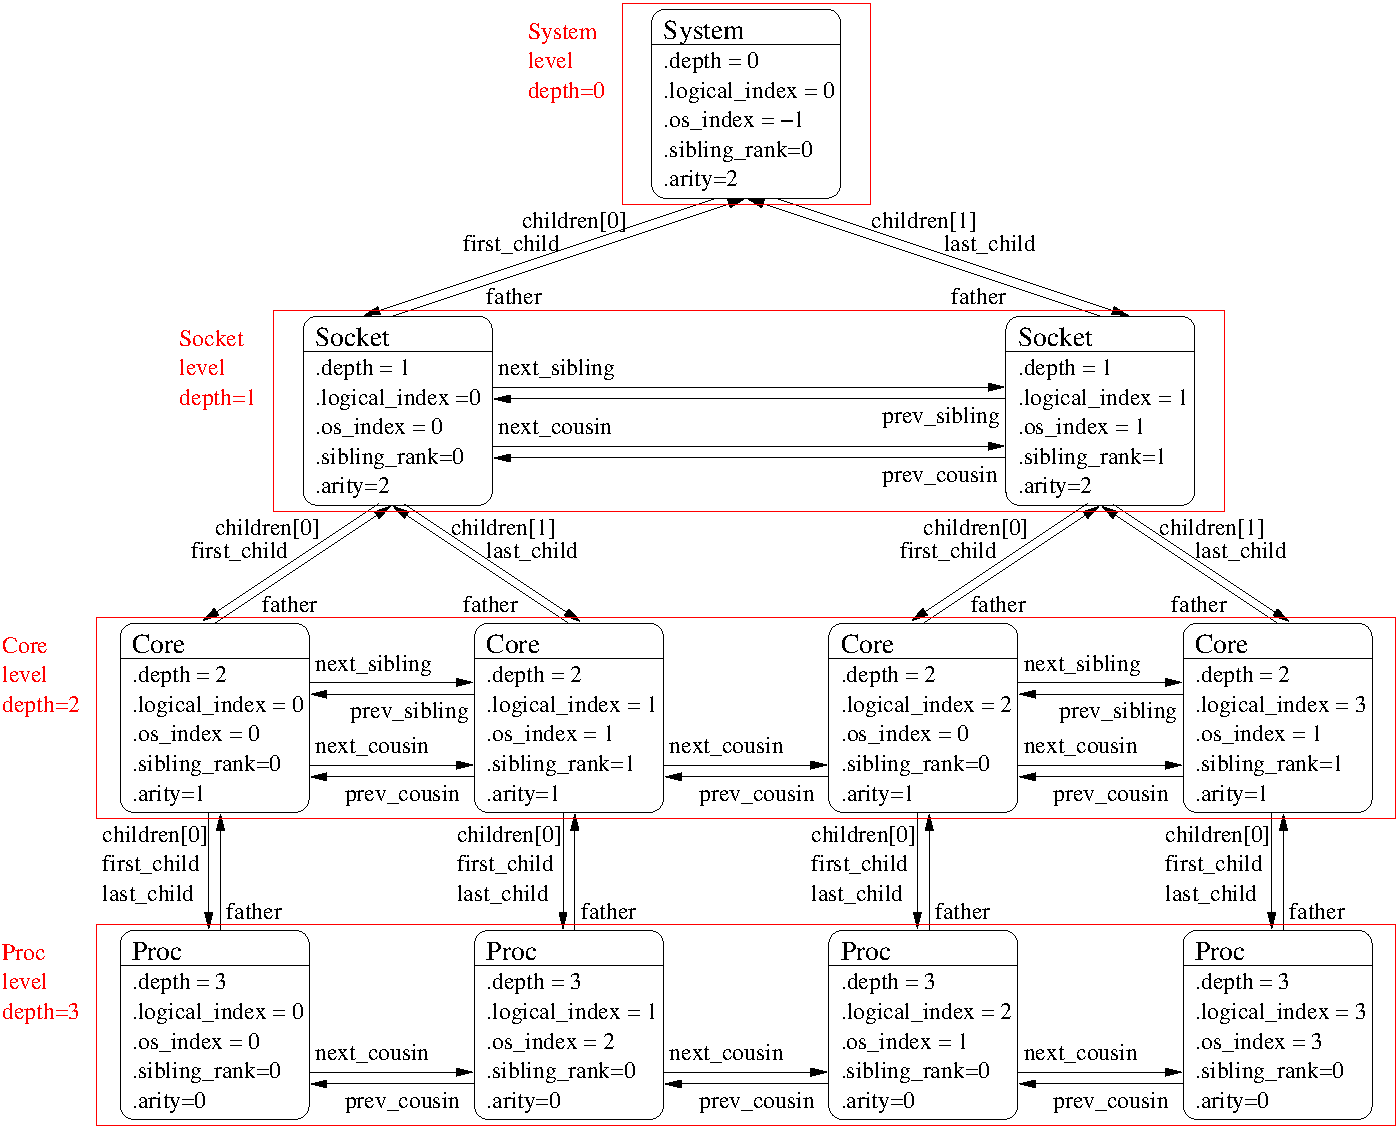
\includegraphics[width=\textwidth]{diagram}}
\end{ImageNoCaption}


It can be noticed that for Processor objects, the logical index, computed linearly by hwloc, is not the same as the OS index. 
